% %% %%%%%%%%%%%%%%%%%%%%%%%%%%%%%%%%%%%%%%%%%%%%%%%%%%%%%%%%%%
% step-1.tex
%
% Author:  Mauricio Matamoros
% License: MIT
%
% %% %%%%%%%%%%%%%%%%%%%%%%%%%%%%%%%%%%%%%%%%%%%%%%%%%%%%%%%%%%


%!TEX ROOT=../main.tex
%!TEX ROOT=../references.bib

% CHKTEX-FILE 1
% CHKTEX-FILE 46

\subsection{Paso 1: Configuración del Simulador}%
\label{sec:step1}

Descargue el simulador de \url{https://github.com/kyordhel/RPiVirtualBoards} ejecutando la siguiente línea de comandos:

\begin{Verbatim}[fontsize=\footnotesize]
git clone https://github.com/kyordhel/RPiVirtualBoards.git
cd RPiVirtualBoards
\end{Verbatim}

A continuación instale todas las dependencias requeridas por el simulador usando \emph{pipenv}\footnotemark{}:

\begin{Verbatim}[fontsize=\footnotesize]
pipenv install
\end{Verbatim}

Finalmente, pruebe el simulador ejecutando la siguiente línea:

\begin{Verbatim}[fontsize=\footnotesize]
pipenv run python temperature.py
\end{Verbatim}

Si, por otro lado, no desea mantener el simulador conmo un proyecto aislado, puede instalar los paquetes con \emph{pip} después de clonar el proyecto:

\begin{Verbatim}[fontsize=\footnotesize]
pip install  --user -r requirements.txt
./temperature.py
\end{Verbatim}

Si la configuración es correcta, verá una ventana similar a la de la \Cref{fig:simboard} con los valores de temperatura simulados cambiando.

\begin{figure}[H]
	\centering%
	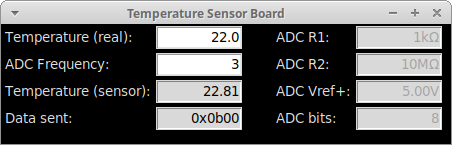
\includegraphics[width=0.5\textwidth,height=8cm,keepaspectratio]{img/simboard.png} %CHKTEX 8
	\caption{Simulador de tarjeta lectora de LM35 con DAC \IIC}%
	\label{fig:simboard} %CHKTEX 24
\end{figure}

\footnotetext{\emph{pipenv} es una herramienta que facilita la creación y administración de entornos virtuales en cualquier proyecto escritos en Python, llevando un control riguroso de los paquetes de los que depende dicho proyecto. Se puede instalar fácilmente con la línea \texttt{pip install --user pipenv}}